\documentclass[a4paper]{danarticle}
\usepackage{a4}
\usepackage[pdftex]{color}
\usepackage[pdftex]{graphicx}
\pagestyle{headings}
\usepackage{amsthm}
\usepackage[pdftex,colorlinks=true,
                      pdfstartview=FitB,
                      linkcolor=blue,
                      citecolor=blue,
                      urlcolor=blue,
		      bookmarks=true
          ]{hyperref}
\pdfinfo{
            /Title      (DoorStep: A system for visitor awareness)
            /Author     (Daniel Hahn)
            /Keywords   (Visitors)
}
\newtheorem*{definition}{Definition}
\sloppy

\begin{document}
  \author{Daniel Hahn}
  \title{DoorStep: A system for visitor awareness}
  \maketitle
  
  \section{Introduction}
    In recent years, the World Wide Web has become more than just a collection
    of static documents, or even a collection of services. It is now perceived
    as a \textit{social space}, where the \textit{netizens} build virtual
    \textit{places}, \textit{visit} each other and engage in all kinds of
    activities.
    
    It can be assumed that the \textit{hosts} of those places would be
    very interested in what is \lq\lq going on\rq\rq\ in their online
    \textit{territory} --- if
    there was a convenient way of monitoring the activity. 
    
    Although
    information about the \textit{visits} is readily available in the
    form of web server logs, the tools for displaying it (e.g. AWStats) will only
    provide statistical information but do not explore the rich context in which
    the visits took place. 
    
    Initial research into the subject by Gellersen and Schmidt\cite{webaware}
    yielded the
    \textit{glances into visitor's sites} approach. They assumed that most of
    the visitors to a site had their own place somewhere on the web, and that
    presenting those places to the host would give him an understanding of the
    kind of \textit{territory} his or her place is in.
    
    In this paper we will take this approach a step further: We will argue that
    even if the visitor does not have an own place (or if we are
    simply unable to find it) she will always have \textit{relations} to various
    places, and in following different types of relations we may be able to
    explore different types of \textit{territories} that in some way adjacent to
    the host's place.
    
    We will introduce a system for finding places that are \textit{related} to
    visitors and will present the results which we gathered from a first
    implementation of this system.
  \section{The DoorStep System}
    DoorStep is a system that attempts to find \textit{places} which are somehow
    \textit{related} to \textit{visits}. We assume that each
    of this \textit{places} can be described by an URL of the form described in
    \cite{url}. Furthermore, we will use the naming conventions and definitions
    introduced in \cite{webaware}:
    \begin{center}
    \begin{minipage}{10cm}
    \itshape
    In the web infrastructure, a web place [\dots] is defined as 
    a set of resources in the web. Resources can
    be HTML documents, images, other media objects or arbitrary applications.
    These resources are made available by web servers, i.e. programs that manage
    resources and make them available worldwide through the web protocols. A
    visit to a web place then relates to a request for a resource in the
    designated set. A request originates from a client, i.e. a program the
    visitor uses to specify his request, typically a standard web browser. Web
    servers routinely log requests for resources [\dots]. These server logs
    constitute a rich source on web activity.
    \end{minipage}
    \end{center}
    There are documents (such as \cite{logfile}) that describe in great detail 
    the 
    data available from web server log files. Additionally to
    this \textit{primary} information, data may be gathered from the
    context of the visit: For example, a certain \verb$User-Agent$ header 
    may indicate a certain type of visitor (e.g. a crawler or bot), or a visit
    from a visitor in the \verb$.co.uk$ domain can be assumed to come from
    Britain. Both the primary and secondary information may be used for finding
    relationships.
    \subsection{System overview}
      The system has three processing steps: Once a visit is received,
      it will determine an URL that acts as a starting point.
      Then multiple \textit{relation finder} instances will start to
      look for URLs (of places) related to the starting place. In
      the final step, the system will take all these URLs and assign an
      \textit{rating} to them in order to mark out the places
      which are the most interesting for the user. The results (ie. the
      rated URLs) are then passed on to be displayed.
      \begin{figure}[h]
        \centering
	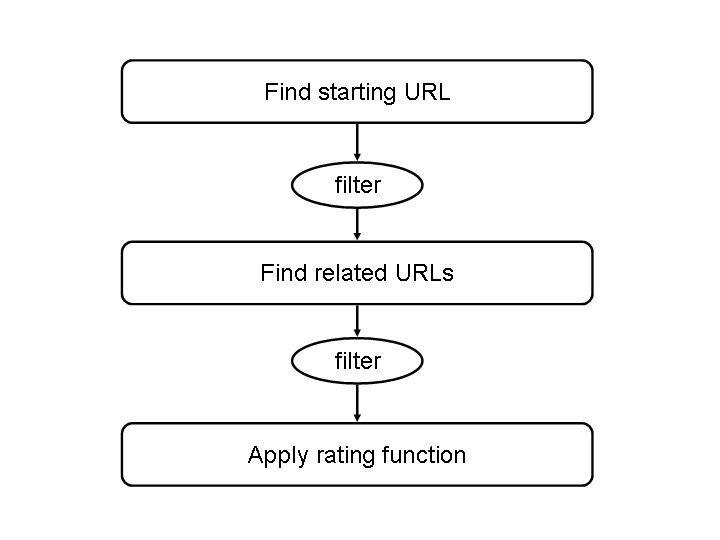
\includegraphics[width=10cm]{steps_overview}
	\caption{Major processing steps of DoorStep}
	\label{steps_overview}
      \end{figure}
    \subsection{Finding a starting place}
       \begin{figure}[ht]
       \centering
	 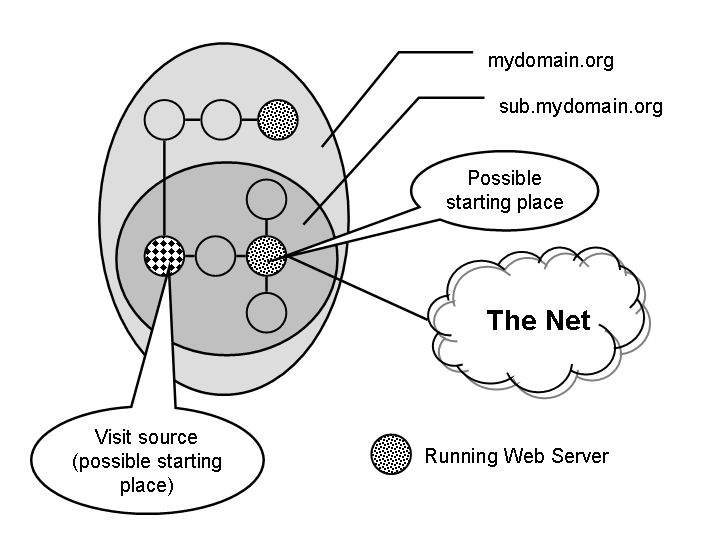
\includegraphics[width=10cm]{startingplace}
	 \caption{Selecting a starting place}
	 \label{startingplace}
       \end{figure}
       The processing starts by looking for an URL of \textit{starting place}. 
       The starting
       place will \lq\lq represent\rq\rq\ the original visit in the next step,
       since it is much easier to describe relations between different
       places than between visits and places.
       
       To find an URL that can represent the original visit, we demand
       that it must be \textbf{as close as possible to the origin of the visit}.
       The meaning of \lq\lq close\rq\rq\ may vary for
       different types of visits, but for visits originating from HTTP requests
       it is reasonably easy to define:
       \begin{definition}
       A HTTP request is closest to the URL describing the address of the
       client.
       \end{definition}
       This starting place may, however, have the drawback of not really 
       being a
       \lq\lq place\rq\rq in the sense that no server is running at the
       address, and thus no resources will be served from there. (the place/URL 
       is not \textit{alive}.) This may or may not be a problem in
       the following processing, so we present an alternate definition of
       \textit{close} that can be used if the starting URL has to be
       \textit{alive}:
       \begin{definition}
       A HTTP request from a given DNS host is closer to URLs in the same
       sub domain than to those in a different sub domain. (e.g. 
       \verb$myhost.banana.hoogla.de$ is closer to 
       \verb$otherhost.banana.hoogla.de$
       than to \verb$otherhost.hoogla.de$, which in turn is still closer than
       \verb$alien.alien.org$).
       \end{definition}
       Of course this definition of close requires that the client has a valid
       DNS host name. If this is a not the case, 
       one can define hosts in the same IP
       subnet as \textit{close}, but it is very unlikely that hosts without an
       DNS host names will be interesting places anyway.
     \subsection{Finding related places}
       The central step is to find URLs that are \textit{related} to the
       starting URL. 
       \begin{definition}
       Two URLS $ u_1 $ and $ u_2 $ are \textit{related} 
       ($ u_1 \leftrightarrow u_2 $) if they \textit{have a common
       characteristic} $ c $. 
       \end{definition}
       Mathematically speaking, $ \leftrightarrow $ is an equivalency relation,
       and both $ u_1 $ and $ u_2 $ are part of the equivalency class 
       $ U_{\leftrightarrow} $
       (of all URLs related by $ \leftrightarrow $). The definition makes no
       further assumptions about the characteristic $ c $, which can be selected
       by the user. Real-life relations of URLs could be things like 
       \lq\lq Both URLs are in the same DNS domain\rq\rq\ or \lq\lq The
       resources served by the URLs contain the keywords a and b\rq\rq . 
       
       For obvious practical reasons it is suggested that relations should also
       fulfil the following criteria: I must be reasonably easy to determine if
       two URLs are related or not and it be reasonably easy to find a
       substantial subset of $ U_{\leftrightarrow} $. 
       \\
       \begin{figure}[h]
         \centering
	 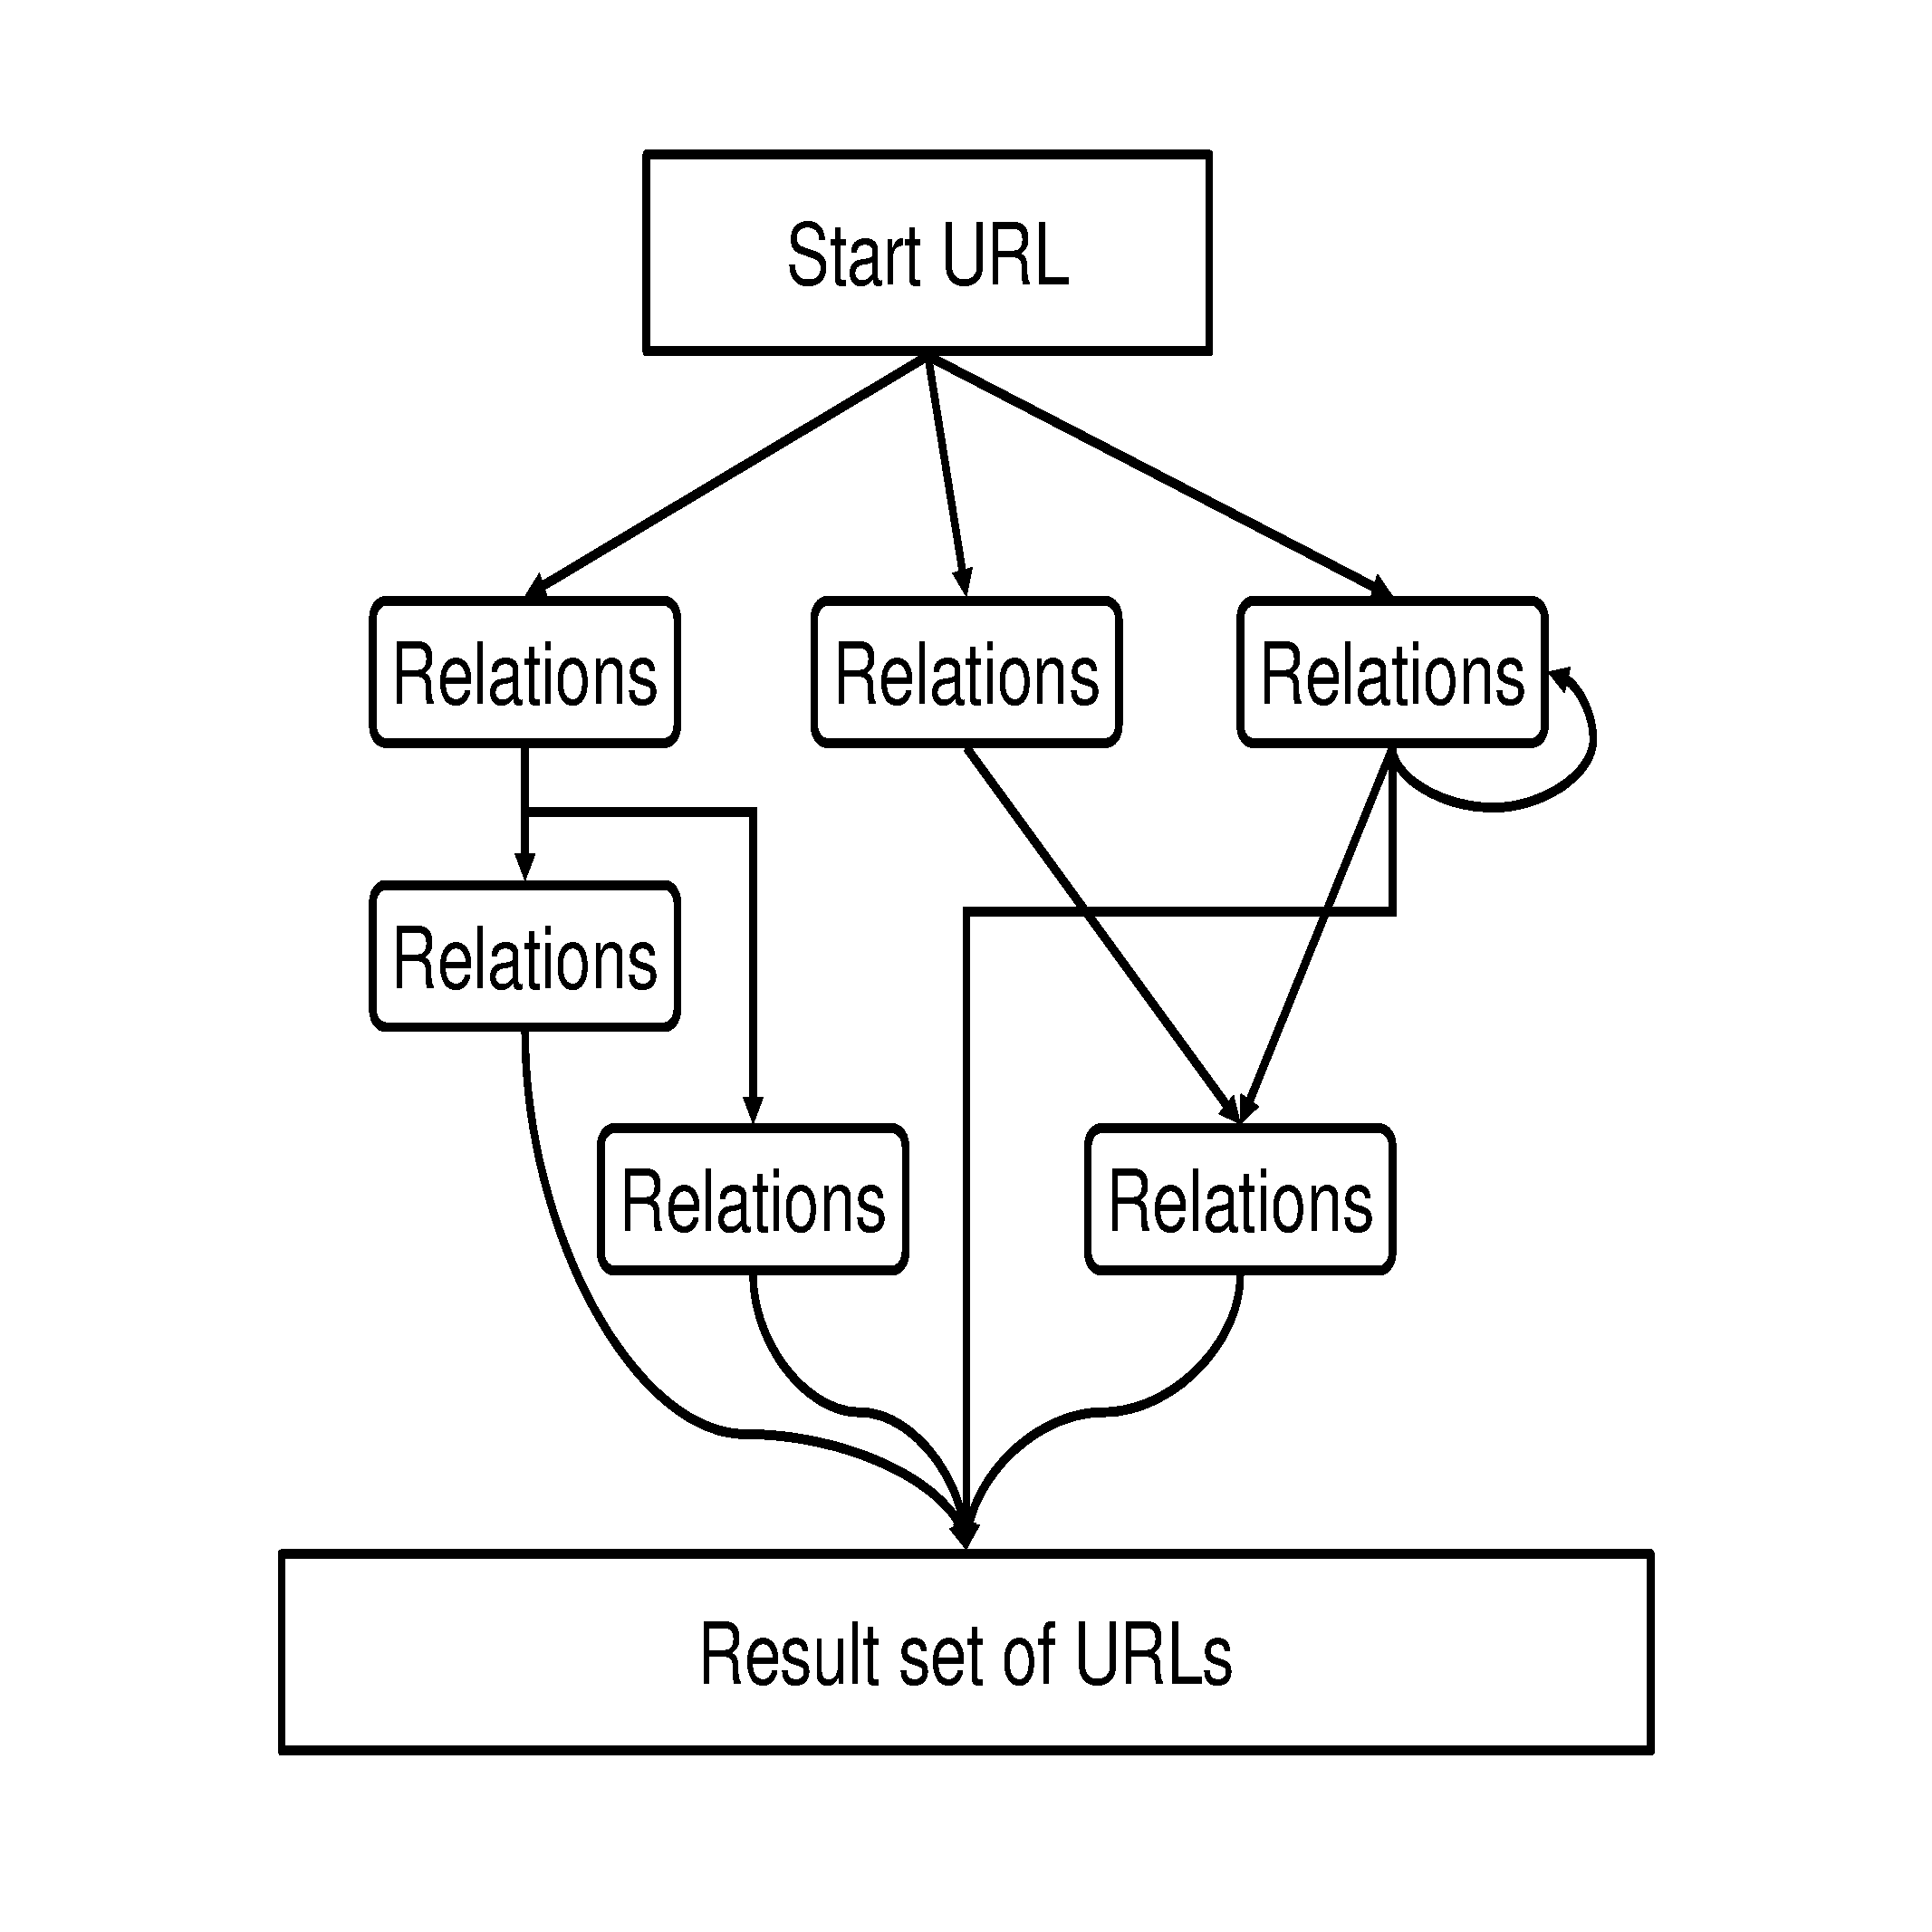
\includegraphics[width=10cm]{relations}
	 \caption{Data flow through different relation finder instances}
	 \label{relations}
       \end{figure}
       To actually find related URLs the system will use a number of
       \textit{relation finders}. Each of those is an object that will take a
       URL $ u $ and tries to find a set of URLs related to it by some relation
       $ \leftrightarrow_{x} $. It is not necessary that a relation finder
       finds \textit{all} the URLs related to $ u $, a subset 
       $ U_{\mbox{found}} $ will
       suffice. (It is $ U_{\mbox{found}} \subseteq U_{\leftrightarrow_x} $.) 
       Since the original URL $ u $
       is related to itself it will also be in the output: 
       $ u \in U_{\mbox{found}} $.
       
       A system may contain different relation finders for different relations. 
       During the
       relation finding process each relation finder may either pass it's output to
       any other relation finders (including itself) \textit{or} to
       the output, allowing for a very flexible setup (Figure \ref{relations}). 
     \subsection{Degrees of relationship}
       \begin{figure}[ht]
       \centering
	 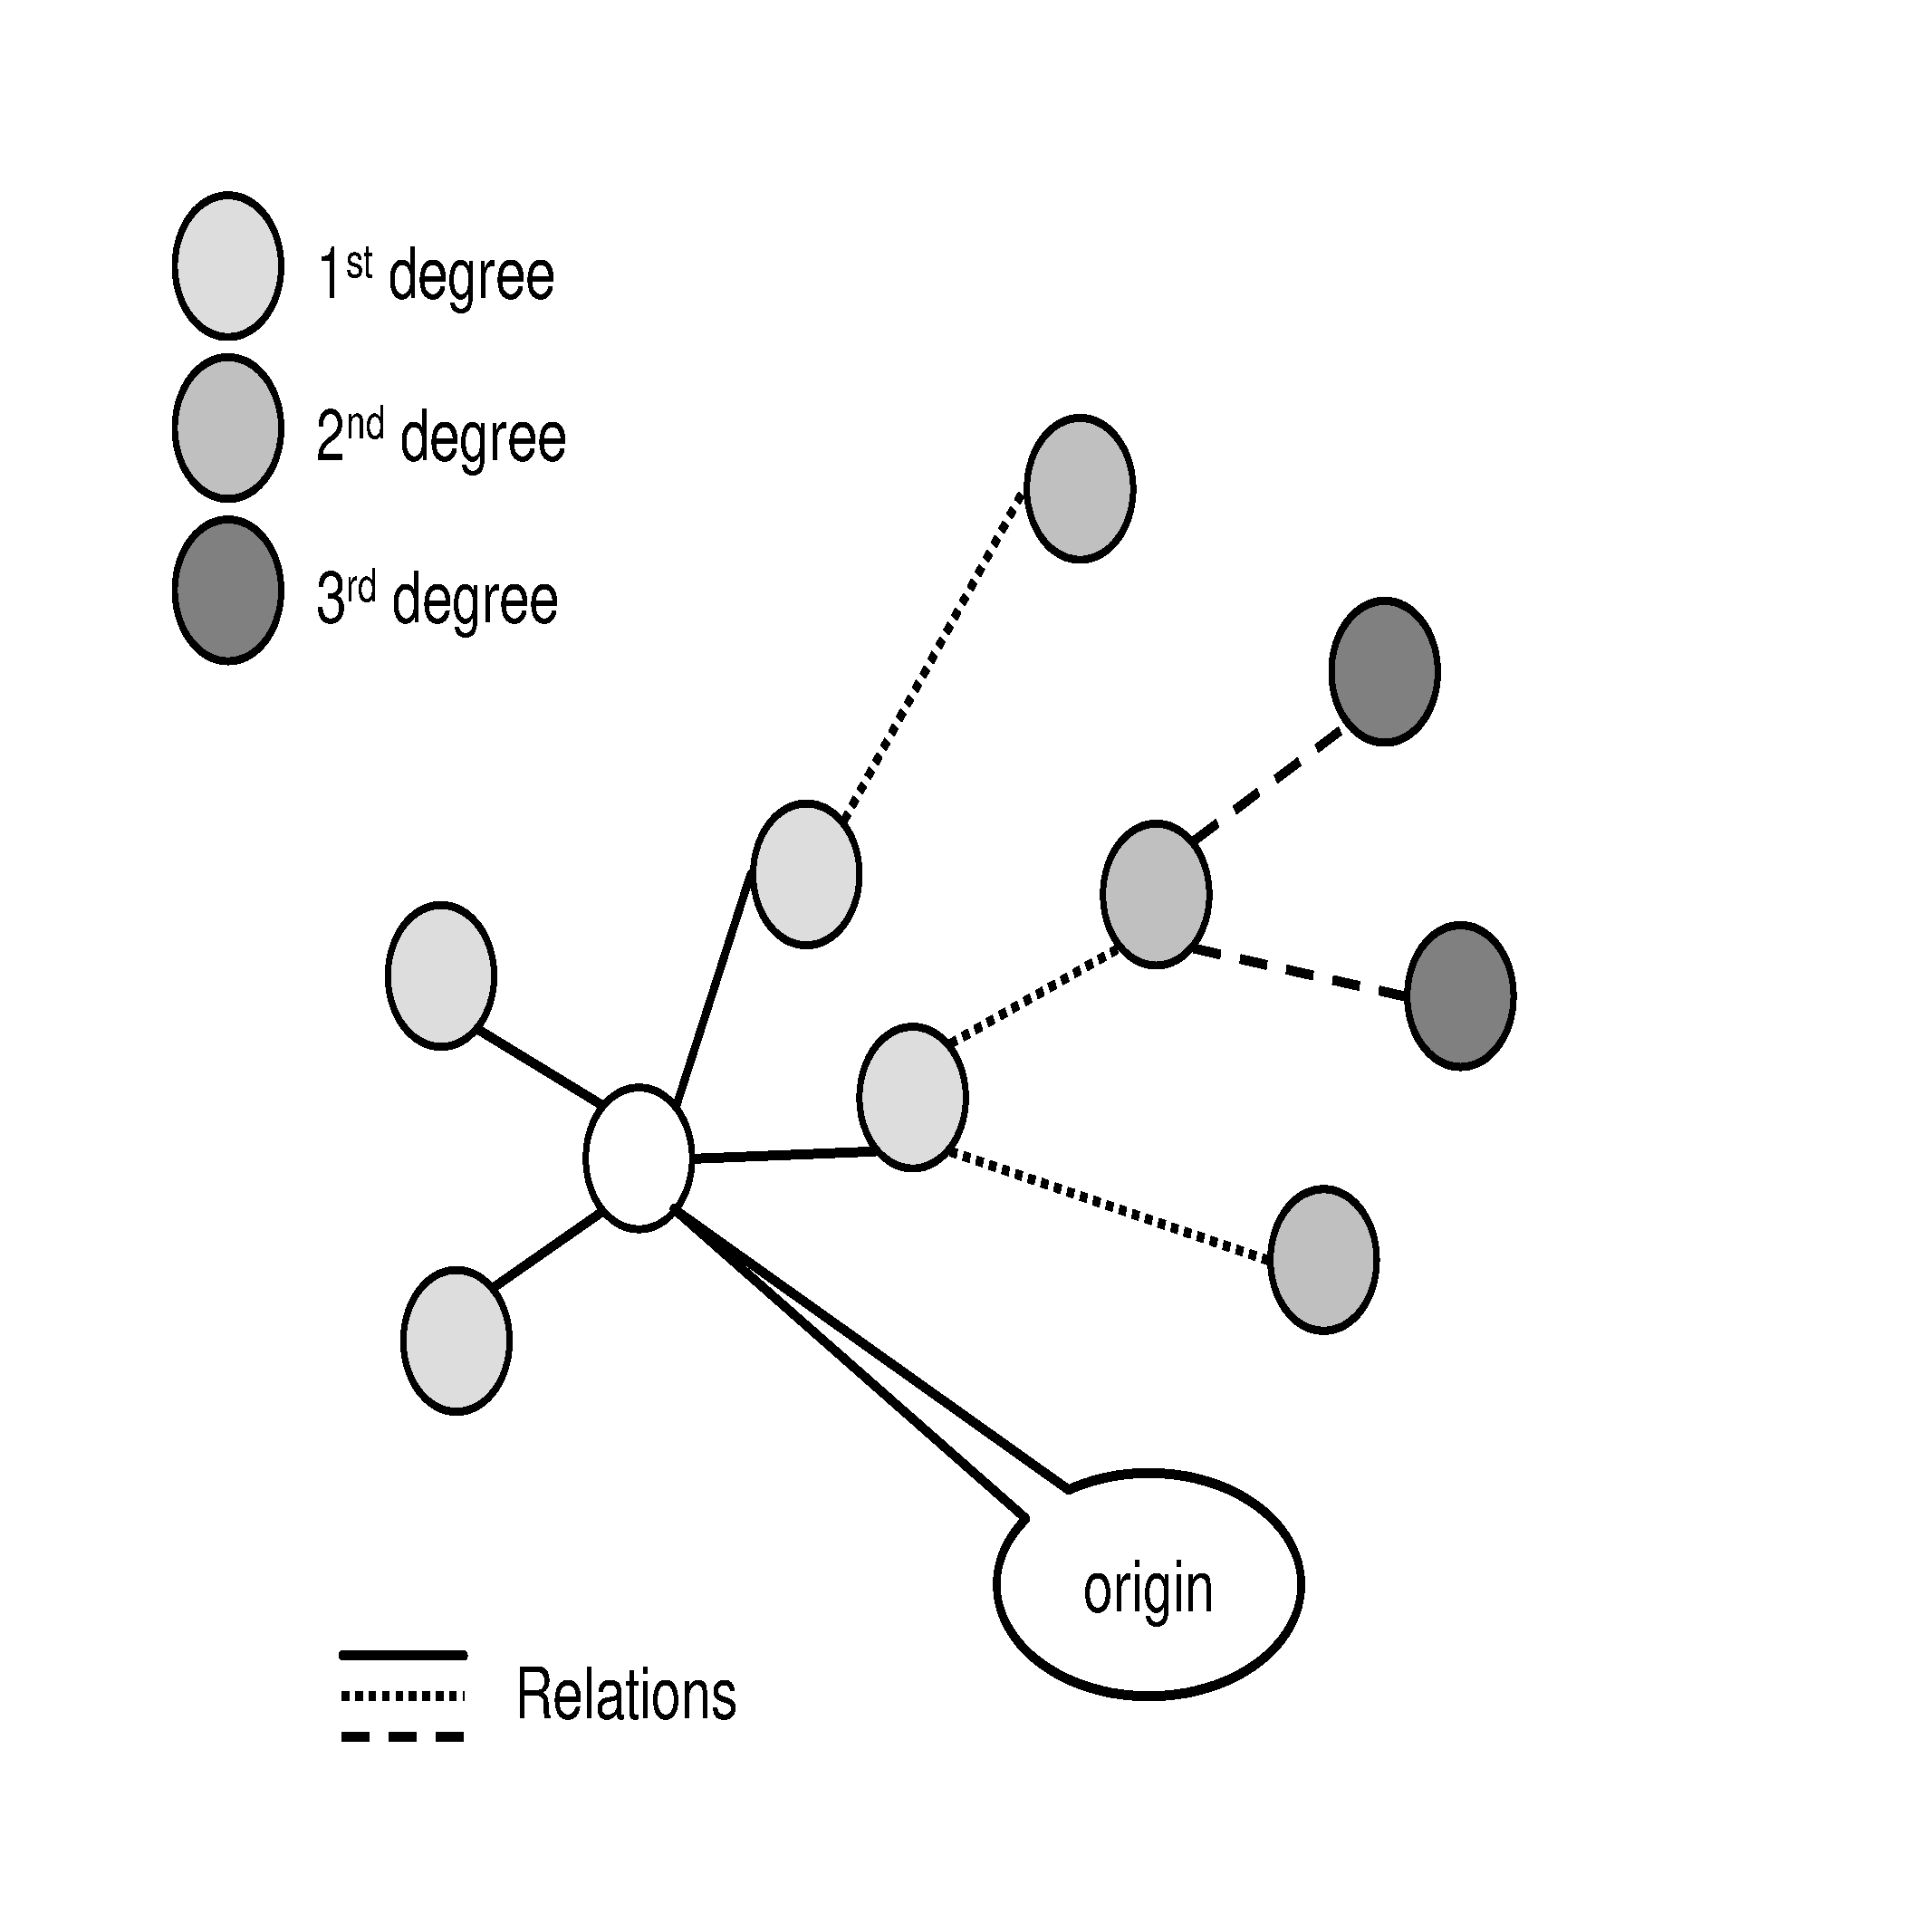
\includegraphics[width=10cm]{degrees}
	 \caption{Degrees of Relationship}
	 \label{degrees}
       \end{figure}
       The flexible setup of the relation finders means that the resulting 
       URLs may have
       different \textit{degrees} of relationship to the start URL. 
       \begin{definition}
       If two URLs $ u_a $ and $ u_b $ are directly related by any given
       relationship $ \bullet $ (i.e. if $ u_a \bullet u_b $), 
       we call them related in the first degree.\\
       Some URL $ u_c $ is called related in the $ n^{th} $ degree to $ u_a $ if
       has no relationship with $ u_a $  but is related to an URL that 
       has a relationship of the degree $ (n-1) $ with $ u_a $. (e.g. if 
       $ u_a \bullet u_b$ and $ u_b \odot u_c $, then $ u_a $ and $ u_c $ are
       related in the second degree)
       \end{definition}
       Thus, the greater the degree of relationship, the \lq\lq farther
       removed\rq\rq\ the URL is from it's relative. The notion of degrees of
       relationship gives us an intuitive measure of the \lq\lq distance\rq\rq\
       from the starting point and has proven to be useful for actual
       implementations of the system.
     \subsection{Rating function}
       Once a set of related URLs is found, one or more 
       \textit{rating functions} will be applied to the URLs. The goal
       of this step is to identify those web places which are the
       most interesting to the user. The concept of \lq\lq interesting to the
       user\rq\rq\ is rather hard to grasp algorithmically, so we will simply 
       say that a URL (or web place) is
       interesting in some aspect $ a $ if it certain properties that can be
       measured through a corresponding \textit{rating function} 
       $ f_a $. The rating of an URL $ u $ regarding this aspect
       can then be expressed as $ 0 \leq f_a(u) \leq 1 $.
       Examples of rating
       functions could be \lq\lq The resource does contain the specified
       keywords\rq\rq\ or \lq\lq The resource contains a text in the user's
       native language\rq\rq .
       
       The system may contain any number of rating functions $ f_1
       \dots f_n $ that measure different aspects that are of interest to
       the user.
       Each of these functions has a weight
       $ 0 < \alpha_i \leq 1 $ which indicates the importance of the given 
       aspect.
       The \textit{overall rating} $ \iota $ of an URL then calculates
       to:
       \[
         \iota(u) = \sum_{i = 0}^{n} 
	 \frac{\alpha_i f_i(u)}{n}
       \]
       An rating value of 1 indicates a most interesting web place
       while a
       value of 0 denotes a very uninteresting one. 
     \subsection{Filtering}
       The system allows for filters to be inserted between the different
       processing steps. A filter will typically check if an URL matches a
       predefined condition and discard it if it doesn't.
       
       Filtering does not change the system in any substantial way but was added
       to remove \lq noise\rq\ and speed up processing.
  \section{Examples of relations}
    These are some examples of relations between URLs that can (or have) been
    used in implementations of the system.
    \\
    
    \textbf{Relation by domain and keywords:} URLs will be called related if
    they are in the same sub domain and are all found by a web search engine
    searching for certain keywords. Instead requiring the URLs to be in the same
    sub domain this kind of relation may also specify that they serve documents
    in the same language or have something else in common.
    \\
    
    \textbf{Relation by links:} Two URLs are related if at least one hyper link
    exists from one of them to the other.
    \\
    
    \textbf{Relation by referral:} Two URLs are related if one of them referred
    a visitor to the other one (note that this is very close to the Relation by
    links).
    \\
    
    \textbf{Relation by referring search query:} Two URLs are related if they
    show up in the result of the same search engine query that referred a
    visitor to one of them.
    \\
    
    The use of web search engines (like Google \cite{google}) is a powerful tool
    and has already been employed in previous research \cite{webaware}. It is an
    easy (and often the only possible) way to find related URLs that may be
    anywhere on the web. 
    
    Each search query on such an engine requires that keywords are given to
    restrict the search. Those keywords may either be statically defined in the
    system or may be dynamically obtained from the web places the system is
    working on.
  \section{Examples of rating functions}
    \textbf{Keywords matching META tags:} This function can be used if the
    resource served by an URL is a HTML document containing tags of the form
    \verb$<meta name="keywords" content="keyword1,keyword2,..." />$ 
    We assume that the users interest is expressed in a list of $ n $ keywords,
    and for each occurrence of one of those keywords in the page's \verb$meta$
    keyword list $ KL $ the rating will be increased by $ 1/n $. Thus
    the rating will be:
    \[
      f_{\mbox{meta}}(u) = \sum{k_i \in KL_u} \frac{1}{n}
    \]
    \\
    
    \textbf{Keywords matching document body:} Especially if the page does not
    contain any \verb$meta$ tags we can try to find the keywords in the
    document's body. Since a word may occur in a page multiple times, we should
    also take the number of occurrences in account. ($ n(k_i) $ is the number of
    occurrences of the keyword $ k_i $).
    
    We will use a weight function $ w $ that assigns a weight to the occurrences
    of each keyword so that $ 0 \leq w(n(k_i)) \leq 1 $ and calculate the
    rating of the URL to
    \[
      f_{\mbox{key}}(u) = \sum_{k_i \in u} \frac{w(n(k_i))}{n}
    \]
    \\
    
    \textbf{Language or Domain match:} The URL is assigned a fixed
    rating if the resource is in a specific language or the URL is a
    specific DNS domain (or something similar).
  \section{System Performance Analysis}
    \subsection{Testbed Architecture}
      In order to evaluate our assumptions, we implemented a testbed that 
      allowed us to test the DoorStep system in a real-life enviroment, using 
      the relations and rating functions given in the examples sections (FIXME: 
      Refer to sections).
      
      The testbed consists of a collection of modules, exchanging XML formatted 
      data: There is one XML format to describe generic \textit{visit events} 
      (Figure \ref{visitxml}) while another is used to describe \textit{web 
      places} (i.e. URLs, Figure \ref{urlxml}). Each module will read XML 
      documents of one of those formats and will produce a document in the URL 
      description format as an output.
      
      
      \begin{figure}[h]
\begin{verbatim}
<visitlist>
  <visit>
    <type>Html</type>
    <timestamp>01:11:2001:00:00:42</timestamp>
    <visitor>
      <class>remote</class>
      <class>agent</class>
    </visitor>
    <resource>/lehre/ubiq/kontext/html/tsld010.htm</resource>
    <host>dudley.waltham.northernlight.com</host>
    <location_code>244</location_code>
  </visit>
  <!-- The file may contain more visits -->
</visitlist>
\end{verbatim}
        \caption{XML format for visits}
	\label{visitxml}
      \end{figure}
      \begin{figure}[h]
\begin{verbatim}
<url_list>
<url>
  <name>http://dudley.waltham.northernlight.com/</name>
  <location_code>244</location_code>
  <timestamp>01:11:2001:00:00:42</timestamp>
  <degree>0</degree>
  <interest>0.5344394</interest>
  </url>
  <!-- The file may contain more URLs -->
</url_list>
\end{verbatim}
        \caption{XML format for URLs (web places)}
	\label{urlxml}
      \end{figure}
      
      The modules will be arranged in a daisy-chain, with a visit-to-url module 
      (called an \textit{extractor} at the head of the chain and any number of 
      url-to-url modules (called \textit{refiners}) following. The contract of 
      an extractor module requires that it finds URLs close to the visits given 
      in the input document (thus performing the first step in the DoorStep 
      processing chain). The \textit{extractor's} output is expected to be a 
      document describing those URLs. The contract of a \textit{refiner} module 
      requires that it acts either as a \textit{relation finder} or a 
      \textit{rating function}. If the \textit{refiner} acts as a rating 
      function it is expected to assign a rating value to each of the URLs on 
      the input. If an URL already has a rating, it shall be modified according 
      to the \textit{refiner's} internal weight. A \textit{refiner} acting as a 
      \textit{relation} finder is expected to read the URLs from the input 
      document and find other places related to them (by a relation that is 
      configured within the \textit{refiner} module).
      
      A \textit{refiner} acting as a \textit{relation finder} can be configured 
      with a maximum degree of relationship. If a URL is encountered with a 
      higher degree of relationship the refiner shall \textbf{not} attempt to 
      find URLs that are related to it -- the URL must be passed on to the 
      output unmodified. This property allows to mimick the flexible setup as in 
      figure \ref{relations} while the \textit{relation finders} are only 
      connected in a simple daisy-chain. (\textit{Refiners} acting as rating 
      functions must ignore the degrees of relationship). It is also required 
      that rating functions must be on the end of the chain.
      
      Each module in the system can contain one or more filters. A filter may 
      remove any entity (visit or URL) from the input \textit{before} any 
      processing is done. The entity will permanently be removed from all 
      processing.
    \subsection{Testbed implementation}
      For practical reasons we created a framework of Java classes that 
      implements the basic functionality of the \textit{extractors} and 
      \textit{refiners}, is capable of handling the connections between the 
      modules and takes care of recurring tasks (e.g. XML decoding or search 
      engine requests). Due to the framework a new module type can (in many 
      cases) be implemented by overwriting but a single method of the 
      framework's superclass.
      
      Nevertheless it is not required that each module is part of the 
      framework or even written in Java at all. As long as a module is able to 
      understand the respective XML format(s) and conforms to the contracts 
      given in the previous section it should be able to interact with all 
      other modules.
    \subsection{User Display}
      The testbed also contains a display architecture that shows a \lq\lq slide
      show\rq\rq of the resulting web pages. The architecture consists of a
      Java-driven web application using servlets and JSPs and requires only a
      standard web browser as a front end. Alternatively, the Display may run a
      small VisualBasic application that is directly driven by a Java server
      process and offers some additional functionality.
      
      The display is meant to run on a separate screen in the user's enviroment
      and change infrequently (i.e. every 2 to 10 minutes) to a new web place.
      If the user is interested in a certain page he has the option to stop the
      slide show and explore that page further (by following the hyperlinks on
      the page). The slide show will automatically commence after a while.
      (FIXME:Pictures)
    \subsection{Test Data}
      The test dataset is part of the HTTP log file from a research lab
      web server. The log file contains about 200.000 entries from a period of
      about 2 weeks.
      
      The file contains a high amount of redundancy and noise: The 200.000 
      entries record visits from only 5720 different clients. Of those, 1603 
      were either visits from local clients (within the same network as the 
      server), failed to retrieve a resource or were requests for pictures 
      within sites.
      
      Most of the remaining entries (82\%) came from a machines with a proper
      DNS host name, and only 18\% from unresolveable addresses -- this indicates
      that methods requiring qualified DNS names should work reasonably well. A
      substantial amount of the entries also carried additional information:
      Almost 40\% of the requests were made by automated agents (e.g. web
      crawlers) that idendentifiable by an \verb$User-Agent$ String and 8\% of
      were referred to the site as the result of a web search (with the search
      string showing up in the \verb$Referer$ field).
    \subsection{Results}
      For the trials we used an \textit{extractor} module implementing the
      metric defined in (FIXME:Reference) to find living URLs, an
      \textit{refiner} module searching the original URLs domain for certain
      keywords and one following the hyperlinks of the original URL. The results
      were rated by two \textit{refiner} modules implementing the rating
      functions given in (FIXME:Reference). The input to the system consisted of
      the 3500 unique and sucessful visits from the original log.
      
      Out of these, the \textit{extractor} module found about 1500 URLs that
      were \textit{alive}. This is a reasonably good set of starting places,
      however a first look at the data revealed that most of them were either
      ISP portal pages or homepages of academic institutions. While the latter
      are in most cases good starting points for further processing, ISP portal
      are rather unspecific and uninteresting in the context of this system.
      This behaviour is mostly due to the fact that many of the \lq\lq
      mundane\rq\rq\ (i.e. non-academic) visitors are \lq\lq homeless\rq\rq\ in
      the sense that the do not have their own web place -- and even if they do
      they often enter the web from a place that is far removed from their own
      place. In a purely academic setting (like ours) this problem is less
      pressing since the user's home place (or -page) is usually loacted within
      the same network from which the user enters the web. This \lq\lq homeless
      user problem\rq\rq\ has already been observed in \cite{webaware}, and some
      solutions have been proposed; this is definitely on of the points for
      further research.
      
      
  \section{Conclusions and Further Work}
     We have shown that the DoorStep system is well suited to show a web host
     his virtual surroundings, and the impressions of the
  \begin{thebibliography}{99}
    \bibitem{webaware} Hans-W. Gellersen and Albrecht Schmidt.
    Look who's visiting: supporting visitor awareness in the web.
    Academic Press, 2000.
    \bibitem{windows} Liechti O, Siefer N and Ichikawa T.
    A non-obtrusive User Interface for Increasing Social Awareness on the 
    World Wide Web. Personale Technologies 3 (1\&2), 1999.
    \bibitem{url} URL RFC.
    \bibitem{logfile} Log file RFC.
    \bibitem{google} Google URL: http://www.google.com/
  \end{thebibliography}
\end{document}
